\section{Allgemein über das Projekt}
\label{cha:ver:sec:Allgemein_über_das_Projekt}

Ähnlich wie ein Desktop-PC, der ein Betriebssystem wie Windows oder Linux benötigt, um seine gesamte Software auszuführen oder die angeschlossene Hardware zu steuern, benötigt embedded Geräte auch  ein Betriebssystem, um ihre Anwendungen einfacher zu verwalten. Das Betriebssystem, das auf unserem Gerät laufen wird, soll also die folgenden 8 Softwaremodule im Hintergrund ausführen, die dann sämtliche Funktionen der IPU-NG Projekt beschreiben. Wie im Kapitel ~\ref{sec:Einl:Ziel_der_Arbeit} beschrieben, sollen im Rahmen dieser Arbeit 3 der 8 unten beschriebenen Softwaremodule in das Betriebssystem eingebaut werden. 
 
\begin{itemize}
	\item \textbf{System Watchdog}: der zuständig ist das System zu überwachen.
	\item \textbf{Power Manager}: der bedient die Stromversorgung der einzelnen Teile des Systems.
	\item \textbf{System Updater}: der aktualisiert das gesamte System, in falls, dass es Neuerung gibt. 
	\item \textbf{License Manager}: 
	\item \textbf{Web Backend}:der dient als Brücke zwischen der Web Anwendung und dem Rest des Systems
	\item \textbf{Web Anwendung / WEB Frontend}: Die Webanwendung ermöglicht es dem Benutzer, den Status des Geräts abzurufen, es zu aktualisieren, die Debug-Protokolldateien
	herunterzuladen
	\item \textbf{System Logger}: die von Linux erzeugten Log Files verfolgen, parsen und entsprechend der
	Liste von oben die notwendigen Informationen von den entsprechenden Log Files extrahieren und in den von der
System Logger Anwendung verwalteten zirkularen Buffer schreiben. 
	\item \textbf{Hauptanwendung}: die stellt die Kern-Funktionalität des IPU NG Gerätes zur Verfügung
\end{itemize} 

Weiterhin sollte im Rahmen dieser Arbeit das Betriebssystem so konfiguriert werden, dass der MCP251xFD CAN-Controller über SPI  sowohl konfiguriert werden als auch Daten  an den Mainline-Linux-Kernel senden kann. 

\begin{figure}[h]
	\begin{center}
		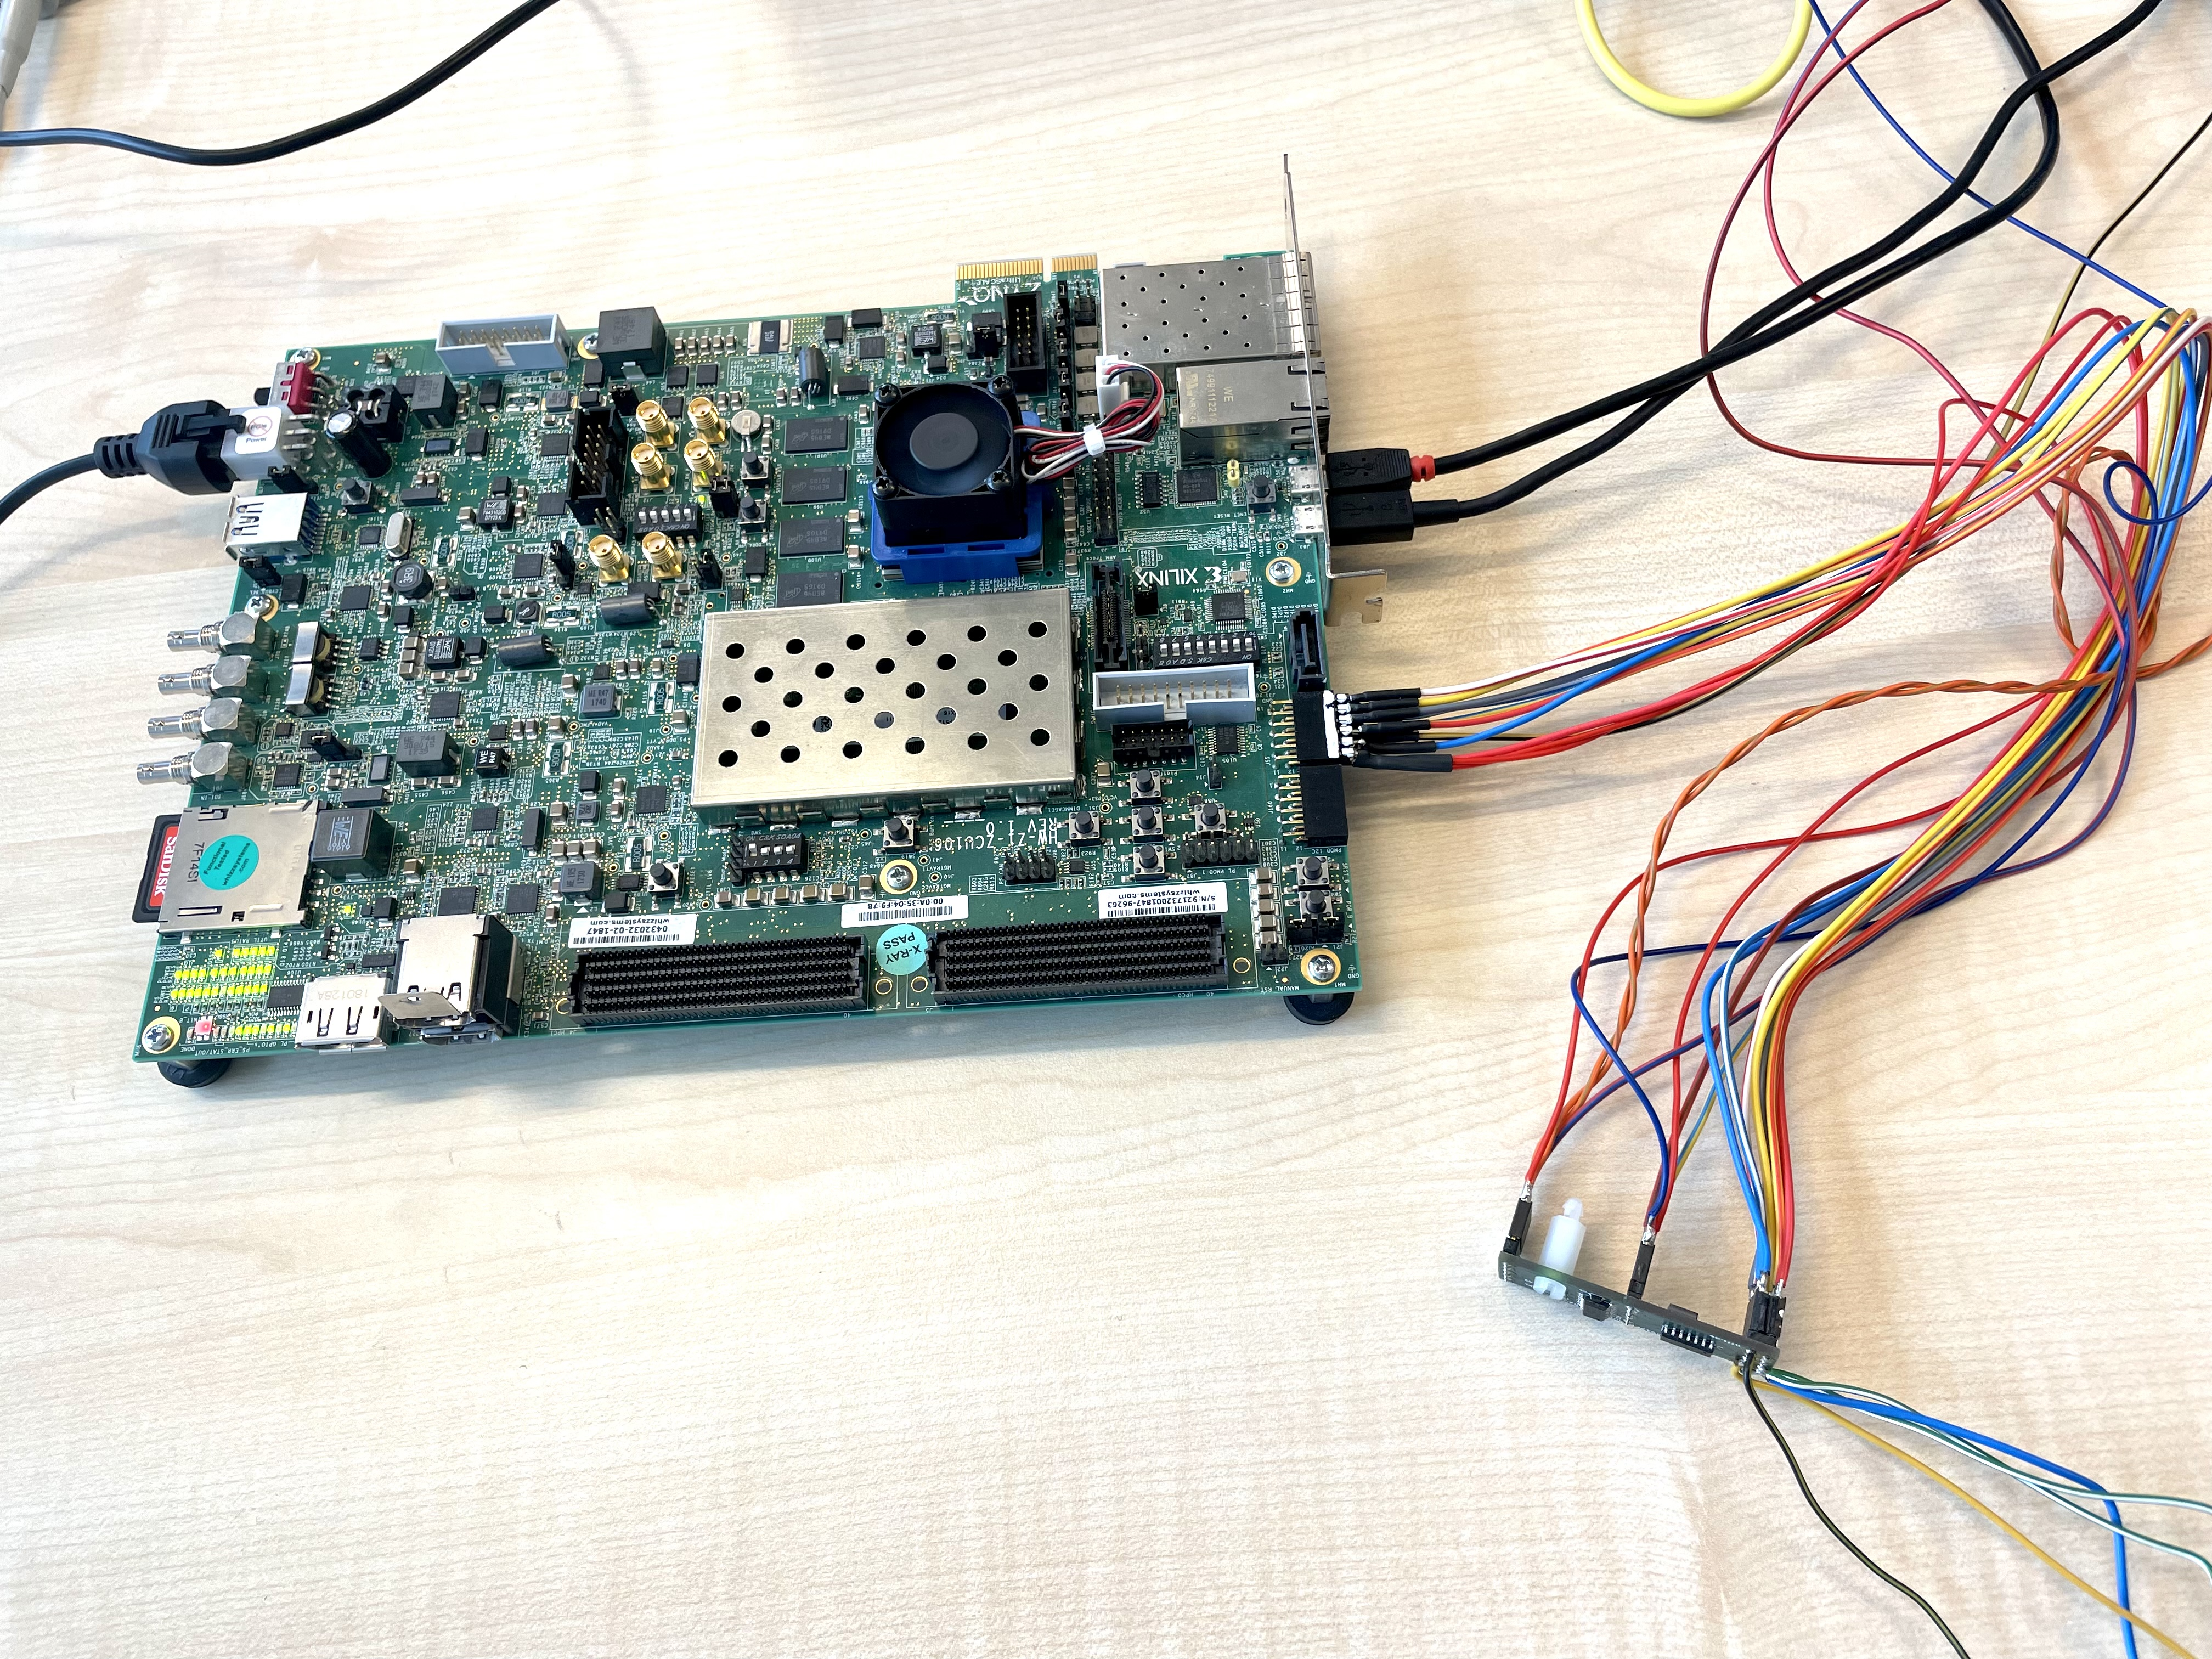
\includegraphics[width=1\textwidth]{./images/Zynqmp_and_mcp.jpg}
	\end{center}
	\vspace{-5pt}
	\caption[Versuchsaufbau ZynqMP Ultralcale + mcp251xfd]{Versuchsaufbau ZynqMP Ultralcale + mcp251xfd} % Eckige Klammer (optional): Caption-Text in Abbildungsverzeichnis
	\label{fig:zynqmp:and:cancontroller}
	\vspace{-5pt}
\end{figure}

Die Abbildung ~\ref{fig:zynqmp:and:cancontroller} zeigt die Verschaltung zwischen der Ersatz Board und der MCP251xfd CAN Controller und der Ersatzt Board Zynq Ultrascale. Im folgenden Abschnitt würde ich eine ausführliche Beschreibung der verwendeten Hardware vorstellen.  